
                \begin{figure}
                    \centering
                    \begin{tikzpicture}
                        \pgfplotsset{%
                            width=1\textwidth,
                            height=0.4\textheight
                        }
                        \begin{axis}[
                            xlabel={Start temperature},
                            ylabel={Average dynamic energy (watt)},
                            ymin=0,ymax=100,
                        ]
                        
                            \addplot [mark=none, densely dashed, red]  coordinates {
                            (35, 18.18590732616388)(40, 18.369287564448882)(50, 48.31343436330823)
                            };
                            \addlegendentry{WRK - IPG}
                            
                            \addplot [mark=none, densely dashed, blue]  coordinates {
                            (35, 20.642332634007122)(40, 17.935803438153563)(45, 18.02230916993157)(50, 18.50229206962415)
                            };
                            \addlegendentry{WRK - LHM}
                            
                            \addplot [mark=none, densely dashed, cyan]  coordinates {
                            (40, 11.70797120825672)(45, 11.84816007499796)(50, 15.810792920870043)(55, 13.290324089319611)
                            };
                            \addlegendentry{WRK - CLAMP (win)}
                            
                        \end{axis}
                    \end{tikzpicture} 
                \caption{A graph illustrating the energy consumption of Cores for test case Nbody with regards to the temperature of the DUT, experiment \#2, (with outliers)} \label{fig:Nbody_Cores_temperature_exp2}
                \end{figure}
                